\documentclass[12pt]{article}
\usepackage[a4paper,margin=2.5cm]{geometry}
\usepackage{tikz}
\usepackage{xcolor}
\usepackage{amsmath}
\usetikzlibrary{arrows.meta,calc}
\definecolor{aksen}{RGB}{247,181,56}

\begin{document}

\section*{Luas Jajargenjang yang Ditemukan dengan Memotong: Alas, Tinggi, dan Bagian yang Digeser}

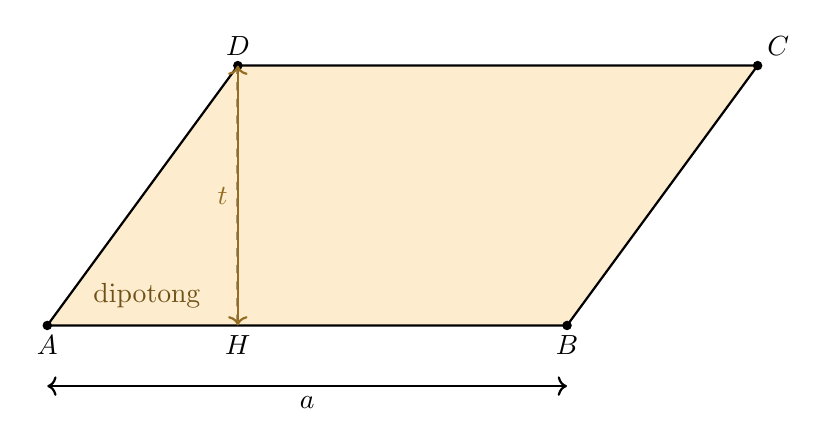
\begin{tikzpicture}[scale=1.1]
  % Panel 1: jajargenjang utuh
  \begin{scope}
    \coordinate (A) at (0,0);
    \coordinate (B) at (6,0);
    \coordinate (C) at (8.2,3);
    \coordinate (D) at (2.2,3);
    \fill[color=aksen!25] (A) -- (B) -- (C) -- (D) -- cycle;
    \draw[thick] (A) -- (B) -- (C) -- (D) -- cycle;
    \draw[dashed,thick] (D) -- (2.2,0) node[below] {$H$};
    \fill (D) circle (0.055) node[above] {$D$};
    \fill (A) circle (0.055) node[below] {$A$};
    \fill (B) circle (0.055) node[below] {$B$};
    \fill (C) circle (0.055) node[above right] {$C$};
    \node[color=aksen!45!black] at (1.15,0.35) {dipotong};
    \draw[<->,thick,color=aksen!60!black] (2.2,0) -- (2.2,3) node[midway,left] {$t$};
    \draw[<->,thick] (0,-0.7) -- (6,-0.7) node[midway,below] {$a$};
  \end{scope}
\end{tikzpicture}

\vspace{1em}
Jajargenjang $ABCD$ dengan alas $a = AB$ dan tinggi $t = DH$, jarak tegak lurus
antara dua sisi sejajarnya. Segitiga sisi kiri ($\triangle ADH$) adalah bagian
yang akan dipindah.

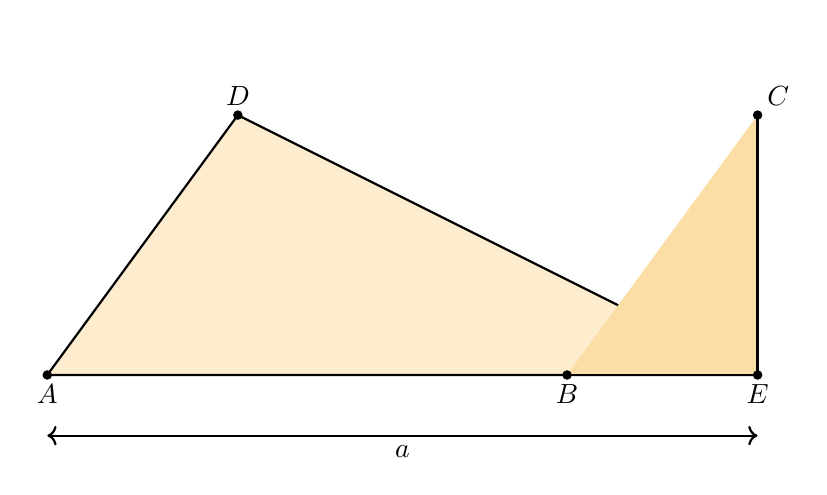
\begin{tikzpicture}[scale=1.1]
  % Panel 2: segitiga dipotong, digeser ke kanan, jadi persegi panjang
  \begin{scope}
    \coordinate (A) at (0,0);
    \coordinate (B) at (6,0);
    \coordinate (E) at (8.2,0);
    \coordinate (C) at (8.2,3);
    \coordinate (D) at (2.2,3);
    % bagian trapesium yang tersisa
    \fill[color=aksen!25] (A) -- (B) -- (E) -- (D) -- cycle;
    \draw[thick] (A) -- (B) -- (E) -- (D) -- cycle;
    % segitiga hasil geser: dari DH ke kanan
    \fill[color=aksen!45] (6,0) -- (8.2,0) -- (8.2,3) -- cycle;
    \draw[thick] (6,0) -- (8.2,0) -- (8.2,3);
    \draw[->,thick,white] (1.1,3.5) -- (5.5,3.5) node[midway,above] {digeser};
    \fill (D) circle (0.055) node[above] {$D$};
    \fill (A) circle (0.055) node[below] {$A$};
    \fill (B) circle (0.055) node[below] {$B$};
    \fill (E) circle (0.055) node[below] {$E$};
    \fill (C) circle (0.055) node[above right] {$C$};
    \draw[<->,thick] (0,-0.7) -- (8.2,-0.7) node[midway,below] {$a$};
  \end{scope}
\end{tikzpicture}

\vspace{1em}
Segitiga $\triangle ADH$ digeser sejauh $a$ ke kanan: titik $A$ tiba di $B$,
titik $H$ tiba di $E$. Hasilnya persegi panjang $AECD$ yang luasnya sama persis,
karena hanya posisi yang berubah, bukan ukurannya.

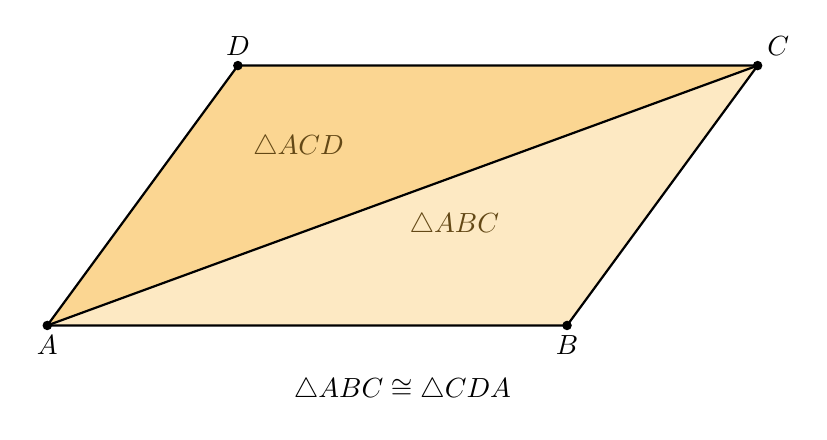
\begin{tikzpicture}[scale=1.1]
  % Panel 3: garis diagonal membagi jajargenjang jadi dua segitiga kongruen
  \begin{scope}
    \coordinate (A) at (0,0);
    \coordinate (B) at (6,0);
    \coordinate (C) at (8.2,3);
    \coordinate (D) at (2.2,3);
    \fill[color=aksen!30] (A) -- (B) -- (C) -- cycle;
    \fill[color=aksen!55] (A) -- (C) -- (D) -- cycle;
    \draw[thick] (A) -- (B) -- (C) -- (D) -- cycle;
    \draw[thick] (A) -- (C);
    \node[color=aksen!40!black] at (4.7,1.15) {$\triangle ABC$};
    \node[color=aksen!40!black] at (2.9,2.05) {$\triangle ACD$};
    \fill (A) circle (0.055) node[below] {$A$};
    \fill (B) circle (0.055) node[below] {$B$};
    \fill (C) circle (0.055) node[above right] {$C$};
    \fill (D) circle (0.055) node[above] {$D$};
    \node at (4.1,-0.75) {$\triangle ABC \cong \triangle CDA$};
  \end{scope}
\end{tikzpicture}

\vspace{1em}
Cara pandang kedua: diagonal $AC$ membagi jajargenjang menjadi dua segitiga
kongruen, $\triangle ABC$ dan $\triangle CDA$. Keduanya beralas $a$ dan
bertinggi $t$, sehingga luas jajargenjang tetap $L = a \times t$.

\end{document}
